\documentclass[specification,annotation]{itmo-student-thesis}

%% Опции пакета:
%% - specification - если есть, генерируется задание, иначе не генерируется
%% - annotation - если есть, генерируется аннотация, иначе не генерируется
%% - times - делает все шрифтом Times New Roman, собирается с помощью xelatex
%% - languages={...} - устанавливает перечень используемых языков. По умолчанию это {english,russian}.
%%                     Последний из языков определяет текст основного документа.

%% Делает запятую в формулах более интеллектуальной, например:
%% $1,5x$ будет читаться как полтора икса, а не один запятая пять иксов.
%% Однако если написать $1, 5x$, то все будет как прежде.
\usepackage{icomma}

%% Один из пакетов, позволяющий делать таблицы на всю ширину текста.
\usepackage{tabularx}

\newcolumntype{L}[1]{>{\hsize=#1\hsize\raggedright\arraybackslash}X}%
\newcolumntype{R}[1]{>{\hsize=#1\hsize\raggedleft\arraybackslash}X}%
\newcolumntype{C}[1]{>{\hsize=#1\hsize\centering\arraybackslash}X}%

%% Данные пакеты необязательны к использованию в бакалаврских/магистерских
%% Они нужны для иллюстративных целей
%% Начало
\usepackage{tikz}
\usetikzlibrary{arrows}
%% Конец

%% Указываем файл с библиографией.
\addbibresource{bachelor-thesis.bib}

\graphicspath{{./media/}}

\begin{document}

\studygroup{K3400}
\faculty{ИКТ}
\specialty{11.03.02~Инфокоммуникационные технологии и системы связи}
\specialization{Программно-защищённые инфокоммуникации}
\title{Разработка программы автоматизированного построения полётного задания для
управления группой БПЛА}
\author{Де Ла Пенья Смирнов Ярослав}{Де Ла Пенья Смирнов Я.}
\supervisor{Карманов Андрей Геннадиевич}{Карманов А.Г.}{доцент, к.т.н.}{}
\programhead{Присяжнюк С.П.}{профессор, д.т.н.}
\publishyear{2020}
%% Дата выдачи задания. Можно не указывать, тогда надо будет заполнить от руки.
\startdate{20}{декабря}{2019}
%% Срок сдачи студентом работы. Можно не указывать, тогда надо будет заполнить от руки.
\finishdate{28}{мая}{2020}
%% Дата защиты. Можно не указывать, тогда надо будет заполнить от руки.
\defencedate{19}{июня}{2020}

%% \addconsultant{}{звание}

%% \secretary{}

%% Задание
%%% Техническое задание и исходные данные к работе
\technicalspec{Требуется спроектировать и разработать прототип программного
обеспечения для автоматизированного построения полётного задания для управления
группой беспилотных летательных аппаратов.}

%%% Содержание выпускной квалификационной работы (перечень подлежащих разработке вопросов)
\plannedcontents{Изучение теории проектирования и разработки систем беспилотных
летательных аппаратов; изучение и анализ необходимых компонентов для
проектирования и разработки программного обеспечения автоматизированного
построения полётного задания для управления группой беспилотных летательных
аппаратов; проектирование и разработка программного обеспечения; описание
архитектуры программного обеспечения.}

\plannedgraphics{Диаграммы, таблицы, рисунки в описательной части; схемы
алгоритмов и листинги кода.}

%%% Исходные материалы и пособия
\plannedsources{\begin{enumerate}
    \item Reg Austin. Unmanned aircraft systems : UAVs design, development and
      deployment;
    \item Douglas M. Marshall и др. Introduction to Unmanned Aircraft Systems;
    \item ресурсы сети интернет: PX4, Gazebo, Cesium, ECMA International.
\end{enumerate}}

%% Аннотация
%%% Цель исследования
\researchaim{Разработать прототип программного обеспечения (ПО) для
автоматизированного построения полётного задания группы БПЛА.}

%%% Задачи, решаемые в ВКР
\researchtargets{\begin{enumerate}
  \item исследовать и изучить предметную область и теоретические основы темы;
  \item определить общие требования к ПО;
  \item выбрать и изучить оптимальные компоненты и библиотеки для реализации ПО;
  \item выбрать оптимальный язык программирования для реализации ПО;
  \item спроектировать и разработать архитектуру для взаймодействия разных
    компонентов;
  \item разработать прототип ПО для построения полётного задания для управления
    группой БПЛА;
\end{enumerate}}

%%% Использование современных пакетов компьютерных программ и технологий
\addadvancedsoftware{Симулятор робототехники Gazebo}{Библиографический список}
\addadvancedsoftware{Автопилот PX4}{Библиографический список}

%%% Краткая характеристика полученных результатов
\researchsummary{<++>}

%%% Гранты, полученные при выполнении работы
\researchfunding{нет}

%%% Наличие публикаций и выступлений на конференциях по теме выпускной работы
\researchpublications{нет}

%% Эта команда генерирует титульный лист и аннотацию.
\maketitle{Бакалавр}

%% Оглавление
\tableofcontents

%% Макрос для введения. Совместим со старым стилевиком.
\startprefacepage

Последние годы уровень развития технологий, в том числе информационных
технологий позволило расширить спектр задач в которых применяются беспилотные
летательные аппараты (БПЛА или БЛА). Изначально БПЛА развивались почти
исключительно для военных целей, только с недавних пор они начали
разрабатываться для гражданских, коммерческих и других государственных целей.

БПЛА --- летательный аппарат (ЛА), который выполняет полёт без человека на борту.
Полётом можно управлять удалённо с наземной станции, либо же в полностью
автоматическом режиме по заранее заданным траекториям или другим
параметрам.\cite{austin-uas}

БПЛА обычно обладают теми же самыми элементами как и обычные ЛА, отличаясь лишь
в отсутствии экипажа на борту летательного аппарата. Другие элементы, то есть ---
запуск, посадка, возвращение, коммуникации, поддержка, и т.д. имеют свои аналоги
и в пилотируемых и в беспилотных ЛА.

Разные виды БПЛА имеют разную степень автономности в зависимости от способностей
ЛА и от требования к задачи. Среди разных видов управления БПЛА в зависимости от
автономности или автоматизированности есть\cite{douglas-intro-to-uas}:

\begin{itemize}
  \item полностью ручное --- когда оператор управляет БПЛА напрямую манипулируя
    движением и траекторией ЛА;
  \item стабилизированное --- когда оператор подаёт команды для управления БПЛА и
    эти в свою очередь обрабатываются автопилотной или компьютерной системой на
    борту и преобразуются в нужные действия;
  \item автоматизированное --- в автоматизированном способе управления оператор
    обладает косвенным контролем над БПЛА, задавая нужные параметры полёта во
    время полёта или заранее составляя полётное задание. Обычно такой вид
    управления производиться посредством ПО с графическим или иным интерфейсом.
\end{itemize}

Нельзя сразу сказать что у БПЛА всегда есть преимущество или недостаток по
сравнению с пилотируемыми летательными аппаратами (ПЛА). Всё зависит от задачи.
Традиционно использование БПЛА, и других роботизированных машин, относили к
задачам или работам, которые в англоязычном мире принято обозначать DDD -- dull,
dirty and dangerous, что на русский язык переводится как «муторно, грязно и
опасно». Данные критерии до сих пор актуальные, но они больше не являются
единственными, которые решают преимущество БПЛА для конкретной задачи. Следующие
виды задач можно отнести к задачам где у БПЛА существует преимущество:

\begin{itemize}
  \item муторные или скучные задачи --- как в военных как и в гражданских
    отраслях существуют задачи как например, длительное наблюдение, которые
    после определенного времени могут привести к усталости и соответственно к
    снижению сосредоточенности и продуктивности что в последствии приводит к
    потери эффективности задачи.
  \item грязные задачи --- также относящийся к военных и гражданских целей, такие
    задачи как исследование среды для выявления загрязнения, например
    радиоактивной или химической, избегая подвержения риску человека. К тому же,
    деконтаминация летательного аппарата проще в случае БПЛА.
  \item опасные задачи --- если говорить о военных задачах, то один из примеров
    это конечно разведка в территориях оккупированными врагами. В таких случаях
    не только избегания риска людей дают преимущество, но и малогабаритность
    БПЛА усложняют их обнаружение или поражение. В случае гражданских задач, то
    это например исследование линии электропередачи, или в борьбе с лесными
    пожарами. Также можно отметить ситуации с экстремальными погодными
    условиями.
  \item скрытые или тайные задачи --- в связи с тем что БПЛА часто меньше по
    размеру чем ПЛА, то их соответственно сложнее обнаружить. Такая
    характеристика БПЛА полезная когда нужно следить за врагом, таким образом
    чтобы он не знал об этом.
  \item исследовательские задачи --- самые первые БПЛА как раз и использовались
    для исследования и разработки новых авиационных систем. Очень часто
    используются копии новых разработанных прототипов гражданских и военных ЛА,
    в том числе ПЛА, что позволяет их тестировать в реалистичных условиях
    дешевле и с меньшей опасностью.
\end{itemize}

Стоит ещё отметить один большой аргумент в пользу БПЛА, и это экономические
причины. Обычно БПЛА, в тех же самых задачах или ролях, меньше ПЛА по размеру,
что и сказывается на их более низкую первоначальную стоимость. Затраты на
эксплуатацию БПЛА тоже ниже, так как их обслуживать проще и дешевле, они тратят
меньше топлива, и стоимость их хранение меньше. Быстрое развитие информационных
технологии способствовало к значительное снижение стоимости и большей
доступности тех компонентов, которые делают возможным беспилотный режим полёта.

\textbf{Актуальность темы} данной выпускной квалификационной работы
заключается в том что в современном мире всё больше и больше растёт спрос на
беспилотных ЛА и появляются новые применения для них. С ростом спроса на БПЛА
появляются новые задачи где требования к возможностям беспилотных систем
меняются и усложняются. Уже не является достаточным запуск одного аппарта и его
управления с наземной станции. Новые задачи требуют больше автономности, не
только в рамках заданного полётного задания, но в том числе способность БПЛА
принимать решения и координировать свои действия с другими БПЛА.

Новые разработки в сфере информационных технологии открывают новые возможности
для дальнейшего развития беспилотных систем для удовлетворения современным
требованиям. В том числе открывается возможность для автоматизированного
построения полётного задания для групп БПЛА.

\textbf{Цель работы} состоит в том чтобы разработать прототип программного
обеспечения (ПО) для автоматизированного построения полётного задания группы
БПЛА. Для выполнения данной цели необходимо решить следующие задачи:

\begin{itemize}
  \item исследовать и изучить предметную область и теоретические основы темы;
  \item определить общие требования к ПО;
  \item выбрать и изучить оптимальные компоненты и библиотеки для реализации ПО;
  \item выбрать оптимальный язык программирования для реализации ПО;
  \item спроектировать и разработать архитектуру для взаймодействия разных
    компонентов;
  \item разработать прототип ПО для построения полётного задания для управления
    группой БПЛА;
\end{itemize}

%% Начало содержательной части.
\chapter{Обзор предметной области и анализ задания}\label{ch:overview}

\section{Обзор систем беспилотных летательных аппаратов}\label{sec:sys-overview}

\subsection{Элементы системы беспилотного летательного
аппарата}\label{subsec:uas-elements}

Начать обзор стоит с системы беспилотного летательного аппарата и каждого
элемента данной системы. Большинство гражданских беспилотных систем состоят из
удалённо пилотируемого ЛА, человеческого фактора, полезного груза, подсистемы
управления, и архитектуры и канала передачи данных и
коммуникаций.~\cite{douglas-intro-to-uas} В военных системах конечно могут
присутствовать и другие элементы, как например оружейные системы.
Рисунок~\ref{pic:diag-elems} более наглядно показывает простой пример системы
БПЛА.

\begin{figure}[!h]
  \caption{Элементы системы беспилотного летательного
  аппарата}\label{pic:diag-elems}
  \centering
  \includegraphics[width=0.9\textwidth]{diag-elems}
\end{figure}

Далее описаны и определены основные элементы системы БПЛА:

\begin{itemize}
  \item \textbf{БПЛА} --- под беспилотным летательным аппаратом подразумевается
    летательный аппарат, управляемый без прямого вмешательства человека внутри
    или на борту данного аппарата. Термин «беспилотный» на самом деле не совсем
    хорошо описывает данные аппараты, поскольку в большинство случаев человек
    всё-таки держит контроль над ЛА, и уровень вмешательства человека в
    управлении БПЛА сильно варьирует от одной системы к другой.
  \item \textbf{Подсистемы управления} --- систему управления можно поделить на
    две части, на бортовую систему управления (автопилот), и на наземную
    станцию управления (НСУ).
    \begin{itemize}
      \item \textbf{Автопилот} --- одно из элементарных возможностей БПЛА это
        выполнение задания минимизируя участие оператора в процессе. Система
        автопилота обеспечивает данную возможность. Степень автономности сильно
        варьируется в зависимости от модели ЛА. Начиная с самых примитивных
        систем где ЛА напрямую управляется оператором и автопилот лишь помогает
        стабилизировать полётные действия, заканчивая с системами где автопилот
        полностью управляет полётом со взлёта до посадки без участия оператора;
        оператор может взять под контроль БПЛА в экстренном случае. В последнее
        время стали массово доступные коммерческие системы автопилота в том
        числе и для малых БПЛА. Многие из этих систем также являются открытыми
        (open source), или предоставляют возможность замена компонентов на
        открытые, позволяя таким образом настроить систему полностью под свои
        нужды.
      \item \textbf{НСУ} --- наземные станции управления предоставляют средства
        для управления БПЛА человеком. Они бывают разных размеров, от ручных
        передатчиков (рисунок~\ref{pic:rc-tx}), до больших объектов которые состоят из
        несколько сооружений с разными приборами и рабочими станциями
        (рисунок~\ref{pic:gcs}).
    \end{itemize}
  \item \textbf{Канал передачи данных} --- этот термин применяется для
    обозначения способа связи между НСУ и автопилотом и описывает как информация
    для управления БПЛА отправляется и получается между ними. Иногда могут
    применяется отдельные каналы связи для коммуникации с системами полезных
    грузов. В отношении радиосвязи, каналы передачи данных можно разделить на
    два вида --- прямой видимости и вне прямой видимости.
    \begin{itemize}
      \item \textbf{Прямая видимость} --- операции или связи прямой видимости
        это прямая связь между НСУ и бортом используя радиоволны. Обычно в
        гражданских БПЛА при радиосвязи прямой видимости используются
        радиочастотные диапазоны 433 МГц, 2,45 ГГц и 5,8
        ГГц.~\cite{avaks-comm-systems} Используемый частотный диапазон будет
        зависит от параметров полёта, используемое оборудование и требований
        полётного задания.
      \item \textbf{Вне прямой видимости} --- связи вне прямой видимости
        производятся обычно с помощью спутниковых коммуникации, или используя
        релейные станции и/или транспорт. Большинство малых гражданских БПЛА не
        нуждаются или не приспособлены к работе вне прямой видимости.
    \end{itemize}
  \item \textbf{Полезный груз} --- за исключением БПЛА, которые служат
    испытательными образцами, большинство БПЛА выполняют определённое задание,
    которое требует наличие полезного груза на борту. Среди  полезного груза
    могут быть приборы разведки и наблюдения; оружие; коммуникационные системы;
    датчики; доставляемый груз или любой полезный груз иной категории. Некоторые
    БПЛА носят полезную нагрузку множество разных категории. БПЛА как правило
    проектируются и разрабатываются в первую очередь с учётом планируемого
    полезного груза, который будет применятся в полётных заданиях БПЛА.
  \item \textbf{Человеческий фактор} --- с каждым днём новые технологии
    позволяют минимизировать участие человека в процессе управления БПЛА. Тем не
    менее, человеческий фактор по сей день остаётся очень важным и неотменяемым
    элементом в системах БПЛА. Данный элемент состоит из оператора (пилота), и
    вспомогательной наземной команды. В зависимости от сложности системы, роли
    могут занимать несколько человек или объединить несколько ролей в одну.
\end{itemize}

\begin{figure}[H]
  \caption{Ручной пульт радиоуправления FrSky X9D Taranis plus 2.4 GHz
  (\url{https://commons.wikimedia.org/wiki/File:FrSky_X9D_Taranis_plus_2.4_GHz_handheld_RC_transmitter.jpg}).
  Автор Enigmasoldier. Лицензия
  \href{https://creativecommons.org/licenses/by-sa/3.0/deed.en}{CC BY-SA 3.0}
  }\label{pic:rc-tx}
  \centering
  \includegraphics[width=0.7\textwidth]{rc-tx}
\end{figure}

\begin{figure}[H]
  \caption{Внутри НСУ беспилотника RQ-7A Shadow 200
  (\url{https://commons.wikimedia.org/wiki/File:Meingcs.jpg}).
  Автор LucasBosch. Лицензия
  \href{https://creativecommons.org/licenses/by-sa/3.0/deed.en}{CC BY-SA 3.0}
  }\label{pic:gcs}
  \centering
  \includegraphics[width=0.7\textwidth]{gcs}
\end{figure}

\subsection{Применения и перспективы}\label{subsec:uas-applications}

За последние несколько лет, рынок беспилотных систем значительно вырос в
результате повышенного спроса на БПЛА. Глобальный объем коммерческого рынка БПЛА
на 2018 год был оценен в 25,59 млрд. долларов и ожидается его рост до 70,28
млрд. долларов к 2029 году.~\cite{bloomberg-uav-market} Развитие технологий и их
доступность открыли возможность применять данные системы в более широком спектре
задач. В связи с развитием новых технологии сотовой связи, применение БПЛА в
полётов и заданиях вне прямой видимости растёт, поскольку данные виды полётов
становятся экономически целесообразными.

На сегодняшний день, БПЛА применяются в множество разных сфер и индустрий.
Большинство заданий, в которых участвуют БПЛА, визуального характера, то есть,
те в которых применяется видео или фотосъёмка. В последние годы также начинают
набирать популярность полётные задания для доставки небольших грузов на малые
расстояния. Однако, логистика таких полётных задании находится на довольно раннем
этапе разработки, и не все детали таких полётных заданий сглажены.

Примеры самых распространённых видов применения БПЛА:

\begin{itemize}
  \item \textbf{Дистанционное зондирование} --- дистанционное зондирование Земли
    определяется как «получение информации о поверхности Земли и объектах на
    ней, атмосфере, океане, верхнем слое земной коры бесконтактными методами,
    при которых регистрирующий прибор удален от объекта исследований на
    значительное расстояние»~\cite{lomonosov-remote-sensing}. Невозможно
    перечислить абсолютно все задания выполняемые БПЛА которые попадают под это
    определение, однако, стоит выделить следующие
    \begin{itemize}
      \item \textbf{Фотограмметрические задания} --- фотограмметрия это «научная
        дисциплина и область техники, предметом которой является получение
        геометрической и семантической информации об объектах
        фотограмметрической съёмки по их фотограмметрическим
        снимкам»~\cite{gost-photogrammetry}. Иными словами, фотограмметрия
        позволяет нам производить измерения в трёх измерениях используя
        двухмерные снимки снятые с разных ракурсов. Фотограмметрия является
        неотъемлемой частью множества задания беспилотных авиационных систем.
        Самое известное применения --- топографические задания, создания карт
        и дальнейшее развитие геоинформационных систем (ГИС). Также применяется
        для задания где нужно измерить объём объектов или пространств.
      \item \textbf{Управление природными ресурсами} --- БПЛА активно
        используются для охраны природы и окружающей среды. Они применяются,
        например, для контроля лесных пожаров, или для наблюдения диких животных
        чтобы упростить контроль населения.
      \item \textbf{Сельское хозяйство} --- с ростом населения необходимо
        применить более эффективные методы выращивания пищи чтобы гарантировать
        доступность самых элементарных продуктов для людей. Существуют многие
        применения БПЛА в сельской хозяйственности, которые помогают повысить
        эффективность. БПЛА могут примениться для анализа урожая или просчёта
        посева.
    \end{itemize}
  \item \textbf{Промышленное обследование} --- данное применения является
    относительно новым и оно начинает распространяться довольно широко среди
    малых БПЛА. Беспилотники используются для обследования объектов гражданской
    инфраструктуры, как например, пролёты мостов; плотин и дамб; опор линии
    электропередачи. Также применяются для максимального автоматизирования и
    ускорения процесса обследования гражданских пассажирских самолётов, как
    можно посмотреть в рисунке~\ref{pic:uav-inspect}.
  \item \textbf{Воздушная фотография и видеосъёмка} --- если говорить о целях,
    которые не являются ни научными, ни военными, ни правоохранительного
    порядка, то данное из первых и самых распространённых применений малых БПЛА
    в коммерческих целях.
    \begin{itemize}
      \item \textbf{Кинематография} --- кинематографическая индустрия уже долгое
        время пользуется беспилотными воздушными системами для снятия фото и
        видеосъёмок. БПЛА менее затратные чем пилотные ЛА, и позволяют делать
        новые виды съёмок, которые невозможны с другими ЛА, как например, съёмки
        на очень низкой высоте, в том числе с залётом в здание.
      \item \textbf{Маркетинг} --- всякий род рекламы может быть снят с помощью
        БПЛА. Виды с птичьего полёта в определённых случаях помогают продвигать
        продукт, товар или услугу.
      \item \textbf{Журнализм} --- БПЛА предоставляют возможность получения
        информации, которая бы осталась недоступной с других ракурсов.
    \end{itemize}
  \item \textbf{Разведка} --- исторический сложилось что такой вид деятельности
    ассоциируется с военными операциями, где с помощью военных БПЛА вражеские
    силы тайно обнаруживаются и отслеживаются. Однако, существуют ряд применений
    которые не относятся к военным действиям.
    \begin{itemize}
      \item \textbf{Обеспечение правопорядка} --- правоохранительные органы
        применяют БПЛА в разных задачах, в таких как, надзор и контроль над
        большим количеством людей в массовых мероприятиях, например, митинги; в
        тактических операциях. Актуальным примером является применение БПЛА
        правоохранительными органами некоторых стран и городов мира для
        соблюдения норм социального дистанцирования во время пандемии
        COVID-19~\cite{usatoday-covid}.
      \item \textbf{Поисково-спасательные работы} --- БПЛА позволяют быстрее
        реагировать в экстренных ситуациях. Запуск, особенно малых БПЛА,
        занимает малое количество времени по сравнению с пилотными ЛА.
    \end{itemize}
  \item \textbf{Метеорология} --- БПЛА полезный инструмент для сбора
    метеорологических данных для прогноза погоды и изучения погодных явлений.
    Отличный пример такого применения --- первые беспилотные полёты NASA над
    тропическим циклоном в 2010 году.~\cite{nasa-hurricane}
  \item \textbf{Доставка грузов} --- в 2013 году американский интернет-магазин
    Amazon объявил о намерений использования БПЛА для доставки покупок до адреса
    проживания покупателей.~\cite{cnn-amazon} Amazon не первые кто предлагали
    такую идею, тем не менее, объявление сделано столь крупной компании проявило
    большое впечатление, что заставило других компаний обратить внимание на
    дальнейшее развитие данного направления систем БПЛА.
\end{itemize}

\begin{figure}[!h]
  \caption{Беспилотник обследует пассажирский самолёт в ангаре Air France
  Industries
  (\url{https://commons.wikimedia.org/wiki/File:AFI_05_2017_Donecle_drone_001.jpg}).
  Автор Josselin Bequet. Лицензия
  \href{https://creativecommons.org/licenses/by-sa/4.0/deed.en}{CC BY-SA 4.0}
  }\label{pic:uav-inspect}
  \centering
  \includegraphics[width=0.8\textwidth]{uav-inspect}
\end{figure}

\section{Анализ требований и целей}\label{sec:analreqs}

Перед тем как приступить к проектированию и разработке, необходимо определить
основные требования к ПО.

\subsection{Требования к функциональности}

Далее в списке представлены минимальные требования к функциональности
разрабатываемого ПО:

\begin{itemize}
  \item создание и редактирование полётного задания для одного и более БПЛА;
  \item автоматизированное генерирование полётной траектории;
  \item сохранение полётного задания;
  \item подключение системы управления (автопилот) одного и более БПЛА к ПО;
  \item управление одного и более БПЛА по заданному полётному заданию;
  \item визуализация полётного задания на спутниковой карте Земли;
  \item визуализация полёта БПЛА на спутниковой карте Земли в реальном времени;
\end{itemize}

\subsection{Требования к совместимости}

Данная программа требует взаимодействие много разных компонентов и других
программных решений. Для обеспечения правильной работы ПО необходимо определить
требования к совместимости для того чтобы подобрать компоненты, библиотеки,
язык(-и) программирования и протоколы коммуникации, использующиеся для
разработки и работы ПО, таким образом чтобы они все были совместимы между собой.

Требования к обеспечению совместимости следующие:

\begin{itemize}
  \item ОС для разработки и работы программы должна быть Linux или другая
    UNIX-подобная система учитывая то, что самые крупные и распространённые ПО и
    инструменты для работы с робототехническими системами разработаны нацелено
    на совместимость стандартов UNIX (POSIX)~\cite{ros-documentation};
  \item выбранный язык программирования должен обладать развитой экосистемой, то
    есть обладать большой базой сторонних библиотек и модулей;
  \item компоненты, библиотеки и стороннее ПО должны обладать лицензией
    свободного программного обеспечения с открытым исходным кодом;
  \item ПО системы автопилота должно иметь способность работать в режиме
    программного обеспечения в контуре, позволяя тестировать систему и
    разрабатываемое ПО без необходимости покупки и запуска аппаратуры;
  \item протоколы коммуникаций должны использовать существующие сетевые стеки,
    например TCP/IP, таким образом позволяя использовать уже существующую
    аппаратуру и инфраструктуру;
  \item исходный код ПО должен использовать определённые стилевые правила и
    должен быть прокомментирован и задокументирован;
\end{itemize}

\section{Анализ архитектуры системы управления группой БПЛА}\label{sec:analarch}

Два самые основные элементы в системе управления БПЛА --- НСУ и автопилот. В
данном случае разрабатываемое ПО является частью НСУ (Здесь и далее под ПО
подразумевается разрабатываемое в ходе данной работы ПО). ПО строит полётное
задание и загружает его в бортовой компьютер БПЛА или в автопилот, либо
управляет в реальном времени БПЛА отправляя команды напрямую в автопилот,
позволяя тем самым менять при необходимости полётное задание во время полёта.
Поскольку целью является управление группой БПЛА, то в данном случае одна НСУ
координирует с несколькими автопилотами. В рисунке~\ref{pic:diag-uav-hw} можно
более наглядно посмотреть примерную схему работы системы.

\begin{figure}[!h]
  \caption{Примерная схема архитектуры системы управления группой
  БПЛА}\label{pic:diag-uav-hw}
  \centering
  \includegraphics[width=0.8\textwidth]{diag-uav-hw}
\end{figure}

Поскольку разрабатываемое ПО является прототипом, и его автор не обладает
достаточными ресурсами для покупки необходимой аппаратуры, тестирование будет
совершаться в режиме «программное обеспечение в контуре» (далее SIL, от
английского Software-in-the-loop), где ПО автопилота взаимодействует с
симулятором для получения симулируемых данных датчиков, и для симуляции полёта
БПЛА.

\begin{figure}[!h]
  \caption{Примерная схема при работе автопилота в режиме
  SIL}\label{pic:diag-uav-sil}
  \centering
  \includegraphics[width=0.8\textwidth]{diag-uav-sil}
\end{figure}

\chapterconclusion

Было произведено короткое обследование систем БПЛА, анализ требований и
предполагаемой архитектуры управления БПЛА.

Исходя из сделанного анализа в данной главе можно сделать вывод что системы
беспилотных летательных аппаратов являются перспективной технологией, а также
то, что есть куда развиваться. Одним таким направлением открытым для развития
является управления несколькими БПЛА в ходе одного полётного задания.

Разработка систем для автоматизированного построения полётного задания для
управления группой БПЛА повышает эффективность БПЛА в некоторых задачах, и
открывает возможности для новых применений БПЛА.

Разработка архитектуры ПО требует множество компонентов и стороннего ПО,
которое должно быть совместимым между собой.

\chapter{Проектирование архитектуры системы}\label{ch:designarch}

\section{Выбор необходимых компонентов и инструментов для
разработки}\label{sec:choosecomps}

Все необходимые инструменты и компоненты для разработки программы должны
подобраны таким образом чтобы они выполняли требования и самое важное, чтобы они
были совместимы между собой.

После анализа предварительной архитектуры ПО и исследования доступных
инструментов, библиотек, модулей, и ПО для разработки, были выбраны те,
подходящие по требованиям. Выбранные компоненты приведены в
таблице~\ref{tab:devbibs}.

В качестве языка программирования выбран мультипарадигмальный язык высокого
уровня JavaScript. Выпуск или версия языка использована в данном проекте ---
ECMAScript 2015 (ES6). Данный выпуск не самый современный, однако, он содержит в
себе самые значительные изменения в стандарте языка, и на момент написания
данной работы поддерживается большинством ПО, что поможет обеспечить
совместимость программы.

Особенности языка JavaScript учитаны при его выборе:

\begin{itemize}
  \item де факто стандарт для разработки веб-приложений, делая его самым
    распространённым языком программирования в мире~\cite{stackoverflow-survey};
  \item простота написания программ, что делает его идеальным для создания
    прототипов;
  \item скорость его исполнения по сравнению с другими языками высокого уровня,
    например Python;
  \item большая и разнообразная экосистема с множество разными библиотеками и
    модулями;
\end{itemize}

В качестве ОС разработки и работы выбран Linux. Дистрибутив Ubuntu версии 18.04
Bionic Beaver был выбран исходя из следующих особенностей:

\begin{itemize}
  \item дистрибутив Ubuntu является самым распространённым дистрибутивом Linux;
  \item версия 18.04 является самой последней LTS (долгосрочной
    поддержки) версией Ubuntu на момент начала проектирования и разработки ПО
    (начало 2020г.);
  \item самая распространённая ОС для разработки программных решений в
    робототехники;
  \item все выбранные компоненты поддерживают данную ОС;
\end{itemize}

\begin{table}[!h]
  \centering
  \caption{ПО, библиотеки, протоколы выбраны для разработки
  ПО}\label{tab:devbibs}
  \begin{tabularx}{\textwidth}{L{0.5} L{0.6} L{1.9}}
    \hline
    Компонент & Выполняемая функция & Описание \\
    \hline
    Linux & ОС & Выбран дистрибутив Ubuntu 18.04 для разработки и запуска ПО в
    связи с тем что разработка большинства стороннего ПО нацелено на работу в
    данной ОС. \\
    PX4 & Автопилот & Автопилот PX4 свободное ПО с открытым исходным кодом для
    управления беспилотными летательными аппаратами, поддерживаемый множества
    разных устройств. Проект предоставляет набор инструментов для разработки
    программных решений для работы с БПЛА~\cite{px4-guide}. \\
    MAVlink & Протокол передачи данных & Лёгкий протокол обмена сообщениями,
    специально разработан для коммуникаций между НСУ и БПЛА и между бортовых
    компонентов БПЛА~\cite{mavlink-guide}. \\
    Gazebo & Симулятор & Свободное ПО для робототехнической симуляции и
    тестирования~\cite{gazebo-guide}, совместимое с автопилотом PX4 в режиме SIL
    и HIL. \\
    React & Библиотека для графического интерфейса & JavaScript библиотека для
    написания графических интерфейсов на основе
    веб-технологий~\cite{react-documentation}. \\
    Electron & Фреймворк для графического интерфейса & Данный фреймворк
    позволяет создать нативные программы и приложения с использованием
    веб-технологий~\cite{electron-documentation}. \\
    Redux & Библиотека для управления состоянием & Javascript библотека,
    позволяющая отделить состояние программы от других компонентов и кода
    программы для обеспечения стойкой и надёжный работы программы посредством
    минимизации ошибок в программе, которые бы могли исказить её
    состояние~\cite{redux-guide}. \\
    Cesium & Библиотека для визуализации объектов на карте мира & Платформа для
    визуализации в трёх измерениях геопространственную информацию, с доступной
    библиотекой написанной на языке программирования
    JavaScript~\cite{cesium-documentation}. \\
    \hline
  \end{tabularx}
\end{table}

\subsection{Компоненты для взаимодействия с пользователем}\label{subsec:uicomps}

Графический пользовательский интерфейс (ГПИ) позволяет пользователю
взаимодействовать с программой в удобном и эффективном порядке. Для построения
ГПИ были выбраны библиотека React и фреймворк Electron.

Для данной программы React выполняет главную роль в создании ГПИ. React
предоставляет готовые компоненты для ГПИ, такие как кнопки, меню, контейнеры, и
базовые компоненты для создания новых графических элементов. Все элементы
графического интерфейса обновляются автоматический React-ом при необходимости.
React также предоставляет XML-подобный язык разметки JSX, который упрощает
разработку ГПИ.

Electron служит простой оболочкой над приложением, позволяя запускать
веб-приложение как обычную нативную программу, и выполняя функцию посредника
между ОС и приложением. По сути это своего рода контейнер, который выполняет
работу подобная работе браузера, но притом предоставляя приложению нужные API
для взаимодействия с ОС.

Также используется библиотека cesium для визуализации полётного задания БПЛА и
для их отслеживания в реальном времени на трёхмерной карте Земли. Данная
библиотека предоставляет доступ к ГИС Cesium.

\subsection{Компоненты бэкэнда и ввода/вывода}\label{subsec:infocomps}

Данная часть программы делиться на два основных компонента --- библиотека Redux
отвечающая за состояние приложения, и бизнес-логика программы.

Redux библиотека на JavaScript предназначенная для управления состоянием
приложения. Библиотека довольно маленькая и её API довольно простой. Данная
библиотека позволяет разграничить задачи разных частей программы, в том числе
отделить компоненты ГПИ от бизнес-логики программы. Это позволяет минимизировать
ошибки в коде программы и их влияния на работоспособность программы.

Бизнес-логика отвечает за основной функционал ПО, который предстоит разработать.
В то же время служит в качестве своего рода клея, объединявший всех остальных
компонентов программы.

Для хранения данных в более долгосрочном порядке (на диск) используются
встроенные возможности языка программирования JavaScript и программной платформы
nodejs.

\subsection{Компоненты коммуникаций}\label{subsec:commscomps}

Для коммуникации между автопилотом БПЛА и НСУ -- то есть, разрабатываемым ПО --
необходимо выбрать один протокол или стек протоколов, которые будут совместимы
с автопилотом и с НСУ. Стек протоколов коммуникации будет состоять из
транспортного протокола UDP и протокола обмена сообщениями MAVLink.

Транспортный протокол UDP был выбран вместо TCP из-за его скорость и малой
задержки в связи с отсутствием «рукопожатий». Так же он поддерживается по
умолчанию автопилотом PX4 в режиме SIL и симулятором Gazebo.

Протокол обмена сообщениями MAVLink был выбран исходя из того, что был
разработан с самого начала с целью использовать его для коммуникаций между БПЛА
и НСУ, и между автопилотом и остальными компонентами БПЛА. Сам протокол довольно
простой и лёгок.

\subsection{Компоненты системы управления БПЛА}\label{subsec:uavcomps}

Самый важный компонент бортового управления БПЛА --- автопилот. Однако, в связи
с требованиям, испытания ПО будут проводится используя симулятор. Выбранный
симулятор должен иметь способность работать с выбранным автопилотом в режиме
SIL, в связи с отсутствием настоящей аппаратуры (то есть, борт, компьютер
автопилота, пульт радиоуправления, и т.д.). ПО PX4 и Gazebo были выбраны в
качестве автопилота и симулятора соответственно.

PX4 был выбран по несколько его особенностям. Данное ПО является одним из самых
распространённых программных автопилотов с свободной лицензией и открытым
исходным кодом, что означает что любой человек или организация имеет право без
ограничений делать пользоваться им, делать изменения в исходном коде, и
распространять копии данной программы. Его популярность также значит что
существует немалое количество аппаратного обеспечения автопилота совместимо с
PX4.

При выборе PX4 в качестве автопилота была возможность использовать разные ПО для
симуляции. Gazebo был выбран исходя из несколько причин. Одна из них, наличие
достаточного количества документации в сети интернет, что облегчает работу с
ним. Также был выбран данный симулятор, по скольку он обладает хорошей
совместимостью с фреймворком для программирования роботов ROS. Фреймворк ROS не
является существенным или необходимым для реализации данного проекта, однако,
его довольно часто используют при сборке некоторых БПЛА для программирования
определённых функций.

\section{Архитектура}\label{sec:archsys}

При наличии всех необходимых компонентов предстоит проектирование архитектуры.
При проектировании архитектуры необходимо определить каким образом будут
взаимодействовать все компоненты, которые были перечисленные в
разделе~\ref{sec:choosecomps}.

\subsection{Архитектура системы}\label{subsec:archsys}

В первую очередь нужно определить архитектуру системы управления в целом,
включая бортовые системы и разрабатываемое ПО.

Как показано на схеме в рисунке~\ref{pic:diag-arch-sys}, у нас существуют один
или несколько инстанций автопилота PX4 в режиме SIL. Для того что автопилоты
генерировали симулированы данные в ответ на полученные команды от
разрабатываемого ПО, необходимо что бы был симулятор который бы предоставлял
симулированную среду откуда бы автопилот(-ы) могли бы получить получать
симулированы данные от симулированных датчиков. И так каждая инстанция PX4
подключена по протоколу UDP к одной и той же инстанции Gazebo откуда и получает
симулированные данные.

Далее, разрабатываемое ПО, после запуска всех нужных инстанций, подключается к
каждой по транспортному протоколу UDP и обменивается сообщениями с помощью
протокола MAVLink. ПО получает от каждой инстанции автопилота информацию о
каждого симулированного БПЛА, и обратно отправляет команды для управления каждым
БПЛА в зависимости от полётного задания.

\begin{figure}[!h]
  \caption{Схема архитектуры системы управления}\label{pic:diag-arch-sys}
  \centering
  \includegraphics[width=0.9\textwidth]{diag-arch-sys}
\end{figure}


\subsection{Архитектура программного обеспечения}\label{sec:archsys}

Далее будет составлена архитектура самого программного обеспечения.

В рисунке~\ref{pic:diag-arch-prog} показаны основные компоненты программы и как
они взаимодействуют друг с другом. Во первых, программу можно поделить на модуль
коммуникации, модуль ввода-вывода, бэкэнд, и ГПИ.

\begin{figure}[!h]
  \caption{Схема архитектуры разрабатываемого ПО}\label{pic:diag-arch-prog}
  \centering
  \includegraphics[width=0.9\textwidth]{diag-arch-prog}
\end{figure}

\subsubsection{Коммуникации}\label{subsubsec:comms}

Коммуникации с автопилотом осуществляются посредством протокола
обмена сообщениями MAVLink. Для обмена сообщениями протоколом MAVLink
используется MAVSDK для JavaScript, который предоставляет удобный интерфейс
между MAVLink и JavaScript. Модуль далее отправляет полученные сообщения в
бэкэнд в компонент по управлению состоянием, и получает обратно от него
информацию, которую необходимо отправить обратно в нужный беспилотник.

\subsubsection{Ввод-вывод}\label{subsubsec:io}

Довольно простой модуль, который взаимодействует с файловой системой ОС для
осуществления операций ввода и вывода данных. В нём применяются нативные функции
Node.js для работы с файловой системой. Общается с модулем бэкэнда по состоянию,
который при определённом событии вызовет нужную функцию по записи или чтения
необходимой информации.

\subsubsection{Бэкэнд}\label{subsubsec:backend}

Бэкэнд основной модуль программы, который отвечает за обработку информации и
содержит бизнес-логику программы. Данный модуль связывает все остальные модули
между собой.

Компонент который управляет состоянием программы во время её исполнения состоит
из Redux. Всё состояние логики программы манипулируется исключительно
посредством Redux. Redux в свою очередь сообщает о любых изменений в состоянии
остальным модулям.

Бизнес-логика программы состоит из несколько классов и функций, которые
координируют всеми остальными компонентами программы также получают,
обрабатывают и выводят информацию.

\subsubsection{ГПИ}\label{subsubsec:gui}

Функция модуля ГПИ лишь в том чтобы предоставить пользователю удобный интерфейс,
через которого он сможет взаимодействовать с программой.

Компоненты графического интерфейса написаны с помощью библиотеки React. ГПИ
строится с помощью так называемых React-компонентов. Контейнер с вьюером cesium
по сути собственный React-компонент с учётом нужд ПО. React ответственный за
обновления визуальной презентации компонентов по требованиям программы.

\chapterconclusion

В данной главе были выбраны необходимые компоненты для реализации программного
обеспечения. На основе выбранных компонентов была спроектирована архитектура
системы управления в целом и архитектура реализуемого ПО.

\chapter{Разработка Программного Обеспечения}\label{ch:devprog}

\section{Установка и подготовка среды}\label{sec:devenviron}

Перед тем как начать разработку ПО, необходимо подготовить среду для разработки.
Устанавливаются требуемые ОС, библиотеки и стороннее ПО в соответствии с теми
что были выбранный в разделе~\ref{sec:choosecomps}.

\section{Разработка бизнес-логики}\label{sec:devlogic}

\section{Разработка ГПИ}\label{sec:devgui}

\chapterconclusion

%% Макрос для заключения. Совместим со старым стилевиком.
\startconclusionpage

В данном разделе размещается заключение.

\startabbreviationspage

\begin{table}[!h]
  \centering
  \begin{tabularx}{\textwidth}{L{0.5} L{1.5}}
    \hline
    ЛА & Летательный аппарат \\
    ПЛА & Пилотируемый летательный аппарат \\
    БПЛА & Беспилотный летательный аппарат \\
    НСУ & Наземная станция управления \\
    ПО & Программное обеспечение \\
    ОС & Операционная Система \\
    SIL & Software-in-the-loop; программное обеспечение в контуре \\
    HIL & Hardware-in-the-loop; аппаратура в контуре \\
    ГПИ & Графический пользовательский интерфейс \\
    ГИС & Геоинформационная система \\
    API & Application programming interface; программный интерфейс приложения \\
    \hline
  \end{tabularx}
\end{table}

\printmainbibliography

%% После этой команды chapter будет генерировать приложения, нумерованные русскими буквами.
%% \startappendices из старого стилевика будет делать то же самое
\appendix

\end{document}
